\documentclass[11pt, oneside]{book}
\usepackage{geometry}       
\usepackage[parfill]{parskip} 
\usepackage{graphicx}
\usepackage{amssymb}
\usepackage{verbatim}
\usepackage{emptypage}
\usepackage{courier}
\usepackage{wrapfig}
\usepackage{listings}% http://ctan.org/pkg/listings
\usepackage[colorlinks=true, pdfstartview=FitV, linkcolor=blue,
            citecolor=blue, urlcolor=blue]{hyperref}
\geometry{letterpaper}   
\lstset{basicstyle={\small\ttfamily},mathescape}
\pagenumbering{arabic}

\newcommand{\lean}[1]{\texttt{#1}}


% ------------------- Title and Author -----------------------------
\title{Using LEAN Theorem Prover to Teach Formal Mathematics:
Lean-Intro-Topology Library}
\author{Rafael Grenier}
\begin{document}


\frontmatter
\maketitle
\newpage
{
  \vfill
  \LARGE 
  \textbf{Abstract}
  \normalsize

  Interactive theorem provers have become more popular in recent
  years within the field of mathematics, since theorem provers provide
  guarantees of the validity of proofs. Even more
  recently, there have been pushes to use theorem provers in the
  classroom to aid in teaching formal mathematics to undergraduate 
  students. Students and instructors alike benefit from the certainty
  provided by the theorem prover, as students can develop a precise
  logical foundation and receive immediate feedback, and instructors 
  can instantly grade their students' proofs. In 2022, Dr. Kevin Buzzard 
  pioneered a course at Imperial College London in formal mathematics
  using the Lean theorem prover \cite{Buzzard}, and some
  other universities have followed suit with similar programs.
  Continuing in this effort to use theorem provers for teaching mathematics,
  I have developed a library of Lean code entitled 
  ``\href{https://github.com/rafaelgrenier/lean-intro-topology/}{Lean-Intro-Topology}''
  with explanations and exercises designed to guide students through 
  formal reasoning and basic set theory, then practice using that newly
  acquired knowledge to prove some theorems in point-set topology.
  This code library has already seen some academic use as a supplemental
  resource for a graduate-level course in Spring 2024
  on formalizing mathematics at the University of Arizona, which my 
  thesis mentor Dr. Sergey Cherkis taught and I assisted. 
  This paper describes the inspiration for creating my code library, 
  its contents, its development process, and the insights I gathered
  while working on the library and as a teaching assistant.

  \vfill
}
\tableofcontents

\mainmatter
% Activate the following line by filling in the right side. If for example the name of the root file is Main.tex, write
% "...root = Main.tex" if the chapter file is in the same directory, and "...root = ../Main.tex" if the chapter is in a subdirectory.

\chapter{Introduction}

Many undergraduate Mathematics programs require students to take 
a proof-writing course, as proofs insert formal rigor into the 
study of Mathematics. Still, there’s some degree of uncertainty, 
since human error is involved in evaluating the proofs and 
determining their consistency. For 
simpler proofs, the risk of human error is a lesser problem, 
since a discerning eye can quickly catch holes in a faulty proof. 
Nonetheless, grading the quality of a slew of proofs is 
time-consuming, especially when factoring in the time a grader 
might take to provide feedback for the specific errors in a 
poorly-written proof. Students may also have difficulty
determining how much detail is sufficient for the proofs they
write, if they even notice the holes in their proofs. For 
both instructors and students, the ambiguity in what constitutes
a ``formal proof'' adds work outside of the mathematical and 
logical focus of the course.

Theorem provers and proof assistants can help resolve this ambiguity,
using the determinism of computing. Theorem provers verify that
the proofs encoded in the prover are sound, namely that they follow
from the axioms and rules of inference. The rigorous framework
of formal mathematics is thus supported by automation which can, 
for students, provide immediate feedback, 
and for instructors, grade instantly and without bias.

One such theorem prover, Lean,
uses dependent type theory and the Curry-Howard isomorphism 
to build a programming language capable of defining and proving 
theorems in Mathematics \cite{TPiL}. Lean stands out when compared to other
theorem provers like Coq and Isabelle due to Lean's
extensive math library, Mathlib, and its large active community 
of users. Lean also has a “tactic mode,” wherein all of the 
premises and goals of a proof are displayed 
as they develop throughout the proof, and functions called 
“tactics” can be used to advance through the proofs using 
automation and type inference. Lean’s large user base and 
committed development team have also created a variety of 
supplemental resources for new users to learn Lean and for 
experienced users to reference, most notable of which is 
\textit{Mathematics In Lean} \cite{MIL}.

\textit{Mathematics In Lean} (MIL) was the primary resource I used 
to learn Lean, and I found the textbook to be a smooth
onramp for a student like myself with a few years of undergraduate
math and computer science education. However, I found the textbook
significantly harder to use once the mathematics being introduced 
expanded beyond what I had already studied. For an audience without
much (or any) proof-based mathematics experience, MIL would be 
far too challenging for a first introduction to formal proof.
As an alternative resource, I have developed a throroughly-commented
interactive code library designed to teach undergraduate Mathematics
students the basics of formal proof-writing, set theory, and topology 
with the assistance of Lean \cite{GrenierLIT}. The code library covers first-order logic,
introductory set theory, order and equivalence relations, induction, and
some point-set topology. 

\begin{wrapfigure}{r}{0.5\textwidth}
    \caption{My GitHub Library}
    \centering
    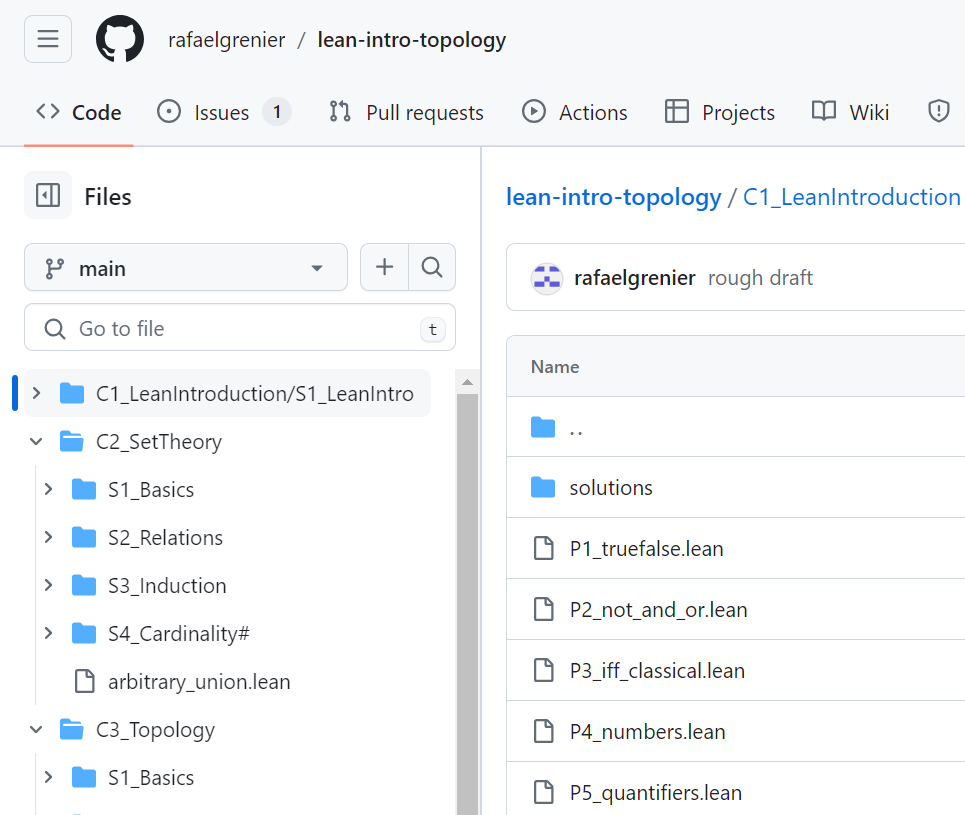
\includegraphics[width=0.5\textwidth]{Chapter1/repo.png}
\end{wrapfigure}

The section \lean{S1\_LeanIntro} of the first chapter \lean{C1\_LeanIntroduction} introduces propositions, 
logical connectives, predicates, quantifiers, and just enough
type theory to begin working with Lean. 

The second chapter \lean{C2\_SetTheory} starts with the section
\lean{S1\_Basics} which introduces sets, set operations like union and intersection,
functions, and cartesian products.
The section \lean{S2\_Relations} considers two kinds of relations:
order relations and equivalence relations. The order relations
discussed are preorder, partial order, lexicographic order, and 
strict order. The introduction to equivalence relations transitions 
to equivalence classes, set/type partitions, and quotients. 
The section \lean{S3\_Induction}
brings in weak and strong induction, as well as inductive
types and recursive definitions.

The third chapter \lean{C3\_Topology} has the final section \lean{S1\_Basics}
on point-set topology which introduces the definition of a 
topology, a topological basis, and open/closed sets. Then the section
pivots to the order, subspace, and product topologies.

This code library was my honors thesis project, and this paper
will explain the structure of the code library, the process of
developing it, and the conclusions I came to as a result.

% Activate the following line by filling in the right side. If for example the name of the root file is Main.tex, write
% "...root = Main.tex" if the chapter file is in the same directory, and "...root = ../Main.tex" if the chapter is in a subdirectory.

%!TEX root = 

\chapter[Development]{Development Process}

This honors thesis project began in June 2023, stemming from
an idea Dr. Sergey Cherkis had for automating the grading
process in his topology class. Over the summer, I endeavored
to learn Lean and become comfortable using Mathlib. In the Fall,
I began building the library, and I finished in the Spring.

\section{Summer 2023}

Lean has many resources available to newcomers, so I began
by tackling the introductory textbooks Mathematics In Lean and
Theorem Proving In Lean. Mathematics In Lean is peppered with
exercises for the reader, which I dutifully completed. When
I read through MIL, it was still written for Lean3, and I only 
covered the sections introducing Lean itself, set theory, and
topology.

The topology section of Mathematics in Lean was sparse, and took 
an approach to Topology centered in the notion of filters. 
\begin{definition}
    A $\mathbf{Filter}\;F$ is a collection of sets over a space $X$
    such that \begin{enumerate}
        \item if $S\in F$ and $\hat{S}$ is a superset of $S$, then
        $\hat{S}\in F$, and
        \item for any two sets $S,T\in F$, then  the intersection $S\cap T\in F$.
    \end{enumerate}
\end{definition}

% MIL's rough introduction to topology inspired me to create an 
% alternate educational resource for topology in Lean.

% I took notes on Theorem Proving in Lean

% I read some of Functional Programming

% Revisited MIL which had been updated to Lean4 in August

\section{Fall 2023}

In Late August, I began to work through the Munkres textbook
"Topological Spaces" with a focus on identifying which parts
of the textbook were more or less challenging to formalize. 
Starting in September, I pivoted to working on the first section
of my instructional repository, Logic in Lean. I spent the first few 
weeks of september deciding how to structure the introduction to 
formal logic, which ultimately culminated in the current path
starting with Propositions, truth and falsity, then leading through
implication, disjunction, conjunction, negation, and the 2 quantifiers.
I actually began writing code and comments in late september, and by
mid-october I had written files explaining proofs, proposition, and
implication; true, false, introduction rules, and elimination rules;
negation; conjunction and disjunction; and the existential and 
universal quantifiers. This was also the time when I began backing 
my files up on github. The remainder of the semester was spent 
continuing to flesh out the library, adding a section on set theory
and a section on Topology.

\section{Spring 2023}

Over the Winter break, it was confirmed by the University of Arizona
mathematics department that Dr. Cherkis would teach a graduate class
in the coming spring, Math 529: Proof Writing and Proof Checking with
a Computer. Furthermore, I was accepted as a Teaching Assistant for
this class. This class gave me the opportunity to discern how 
approachable formalization of Mathematics in Lean is in an actual
classroom environment. During this semester, I also began writing 
this Honors thesis, and I finished working on the code library
which introduces students to Lean. 

\subsection{Finishing the library}

My original plan for the project
included a subsection in the Set Theory chapter of the library for
cardinality which would cover the explicit definitions of finiteness, 
countability, and uncountability, but after several weeks of work on 
the code without any forward progress, I decided to cut cardinality
from the code library. The first roadblock I encountered trying to
formalize Munkres' approach to cardinality was a paralysis of possibility, 
since Lean has finiteness defined for sets and types, each of which are
useful in select situations. Mathlib has the type \lean{Finset}, which is 
built atop Lean's programming infrastructure for lists, so all terms 
of type \lean{Finset} are constructed explicitly by enumerating their 
elements. This extensional finite set construction makes proving theorems about
cardinality all but trivial, but requires some type of external means
to interpret intensionally defined sets as \lean{Finset}s. Mathlib also 
has the type \lean{Fin : Nat $\to$ Type} and the 
predicate \lean{Finite : Type $\to$ Prop}. For \lean{n : Nat}, 
\lean{Fin n} is a subtype of \lean{Nat} consisting of all natural numbers
less than \lean{n}. \lean{Finite} is defined in terms of \lean{Fin}, where
a type is \lean{Finite} if there exists a bijective function from
that type to some \lean{Fin n}. This approach to finiteness matches the formal
approach described by Munkres, but requires introducing extraneous concepts
from the Mathlib library used for the construction of \lean{Finite}, namely
\lean{Equiv} and \lean{Subtype}. I attempted writing some files in the code
library relying on each approach, since \lean{Finset} is actually used 
later on in topology where finite subcovers and finite intersections are 
concerned, but only \lean{Finite} lends itself to the formal proofs of
the uniqueness of cardinality and so on. \lean{Finite} is also most similar
to how countability and uncountability are defined in Mathlib, so it provides
a better segue. However, I was met with another significant hurdle when trying
to prove that cardinality is unique using \lean{Finite}. Extending a function's 
domain to a larger type requires using Lean's if-then-else logic, which
is tricky to use in tactic proofs. Even if the if-condition is met by 
one of the hypotheses, some elbow grease is necessary to convince Lean to
simplify the if-then-else expression. This felt like an unreasonable onus 
to place upon students learning Lean and set theory for the first time, so 
I spent several hours searching for a workaround, but to no avail. 

Ultimately,
I decided to scrap the Countability section, for the sake of producing a 
cohesive code library before the end of the semester. Consequently, I also
needed to drop the Compactness section of the Topology chapter of
the code library. Due to time pressure, I pared down the Topology chapter
even further, leaving only the first section to be written. By April 2024, 
I had finished writing all the remaining code within the limited scope, 
including solutions for all the exercises within the code library.

\subsection{Insights as a TA}

Dr. Cherkis constructed a curriculum for the graduate level course 
which spent the first two months leading students through the first 6
chapters of \textit{Mathematics in Lean}, then took a handful of weeks to 
guide students through my code library, before returning to finish 
MIL in April. The class met twice weekly for 75 minutes, and a typical class
session spent about 20 minutes on lecture, and the remaining time dedicated
to individual or paired work on students' computers with Lean exercises. During
the group and individual work time, Dr. Cherkis and I helped students upon 
request, clarifying concepts or quirks of Lean.

\subsection{Future Development}
% Activate the following line by filling in the right side. If for example the name of the root file is Main.tex, write
% "...root = Main.tex" if the chapter file is in the same directory, and "...root = ../Main.tex" if the chapter is in a subdirectory.

%!TEX root = 

\chapter{Structure}

\section{Introduction to Lean and Logic}

Conventionally, Propositional Logic is taught with a few basic ideas:
A proposition is any statement which can be binarily assigned true or 
false, and every proposition must be either true or false. Next introduced 
are truth tables, and different means of combining propositions into 
larger propositions. We define the meaning of conjunction by appealing to 
a truth table, wherein $P\wedge Q$ is true only if $P$ is true and $Q$ is true.
Similar constructions define negation, disjunction, and implication. 

In Lean, every term has some Type, and true-or-false claims have the type 
$\mathit{Prop}$, which is short for Propositions. Any given term $P$ with
type $Prop$ is itself a type, and a term $hp : P$ is understood to be a 
proof of the proposition $P$. Therefore any function which produces as its
output a term of type $P$ is a means by which $P$ can be proven. This gives 
us a vehicle by which we can conceive of implication! If there is a function
$f$ which takes as its argument some term $hp$ of type $P$ and returns
a term of type $Q$, then $f$ is a term with type $P\to Q$. Provided that 
$P$ and $Q$ are terms with type $Prop$, $f$ can be throught of as a proof
that $P$ implies $Q$. This means of creating implication as a function from
one Proposition to another is known as the Curry-Howard Isomorphism, and
provides the basis for Lean as a proof assistant. 

The above mentioned introductions to logic are very different, so I needed
to make a choice with my code library: Do I use adapt truth tables into
Lean and teach basic logic that way, or do I introduce basic logic through
introduction and elimination rules, as is infitting with how Lean itself 
is organized? I chose to follow the path tread by the structure of Lean itself,
especially because actual mathematical proof typically abandons truth tables
before long. Therefore my code library starts with a brief explanation of
propositions and proofs, where proofs are functions from one proposition to
another. I then introduce tactics and tactic states, the other main feature
of Lean. Tactics make proof-writing in Lean flow more smoothly and resemble 
proof-writing in Human language more than pure functional code. The tactic
state also represents to the reader/writer of Lean code the names of all
hypotheses already known (the function arguments and local variables), as 
well as all the goals of the proofs (the type which the function should return).
Each new tactic employed updates the tactic state, so proving a theorem with
tactics amounts to writing tactics until the tactic state represents that there
are no goals left to be solved. I equip students with knowledge of just 3 basic
tactics in the beginning: $intro$, $apply$, and $exact$.

The $intro$ tactic functions similarly to "let" in a human language proof. 
In some proof about Natural numbers, one might write "let n be a natural number."
Similarly, in Lean, one would write $intro\;n$.
If the current goal in the tactic state is in the form 'P → Q', then
"intro hP" would update the tactic state so that there's a new hypothesis
hP : P and a simplified goal Q. "hP" is an arbitrary name here, whatever
sequence of alphanumeric characters follows the whitespace after "intro" will
be the name assigned to the term introduced. 

The $exact$ tactic is used for finishing off a proof, and might be compared
to the phrase "Because blank, the proof is complete." If the current goal is
"P" and there is some hypothesis "hp : P", then writing "exact hp" would 
complete the proof.

The $apply$ tactic uses implications to change the goal. For example, 
given the goal 'Q' and the hypothesis "h : P $\to$ Q," writing
$apply\;h$ would transform the tactic state such that the new goal
is 'P'. Since it's known that P implies Q, proving P would suffice to 
prove Q, and the apply tactic packages that logic into a single line.

The code library then works through True, False, Not, And, Or, and Iff.
True and False are both propositions, where True.intro is a function which
returns a proof of True and requires no arguments, and False.elim is a function
which takes a proof of False as an input and can output a proof of any
proposition. Not has type $Prop \to Prop$ and is denoted $\lnot$, so for
some Prop $P$, $\lnot P$ is also a Prop. $Not\;P$ is defined as
$P\to False$. $And$, $Or$, and $Iff$ are all terms of Type 
$Prop\to Prop\to Prop$, and are denoted by 
$\wedge$, $\vee$, and $\leftrightarrow$ respectively. These logical connectives
all have introduction and elimination rules; introduction rules for
creating a term with the type of the connective, and elimnation rules for
turning terms with the type of the connective into proofs of other propositions.
For example, $And.intro$ takes proofs of $P$ and $Q$ and returns a proof of
$P\wedge Q$. $And$ has two elimination rules, $And.left$ takes a proof
of $P\wedge Q$ to a proof of $P$, and $And.right$ takes a proof of 
$P\wedge Q$ to a proof of $Q$. 

\subsection{Dependent Types and Qualifiers}

Lean implements "Dependent Type Theory," which allows for the quantifiers
$\forall$ and $\exists$ to be represented in Lean. If $\alpha$ is some
type and $p$ has type $\alpha\to Prop$, \textbf{TBD}

\subsection{Are "to be" are "not to be" the only options?}

Using the the Curry-Howard Isomorphism and defining logical connectives
with introduction and elimination rules creates a system of logic which
is almost as expressive as classical logic, but it has a few shortcomings.
It's not possible to prove $P\vee\lnot P$ for an arbitrary proposition $P$
with constructive logic, the logic we have been using in Lean thus far.
Lean introduces three axioms in order to prove the law of the
excluded middle: propositional extensionality, functional
extensionality, and an axiom of choice. Propositional extensionality is the
axiom that equivalent propositions are entirely equal, functional extensionality
is an axiom stating any two functions which return the same outputs for any
given input are entirely equal, and the choice axiom is a function which produces
an term of an arbitrary type $\alpha$ given that $\alpha$ is a nonempty
type. Then using Diaconescu's theorem, it's possible to show that for any
proposition $P$, either $P$ or $\lnot P$ is true. 

The code library doesn't dwell very long on the differences between 
constructive and classical logic, nor does it discuss the measures
taken by the Lean library to extend its expressive capabilities to 
cover classical logic. The library is geared towards an audience of 
undergradute mathematics majors, so most of the time is spent developing
their understanding of classical logic.


\section{Set Theory}

The structure of the Set Theory section of the code library is modeled after 
\textit{Topological Spaces} by James Munkres and 
\textit{An Introduction to Proof through Real Analysis} by Trench, along with
some influence from the undergraduate course I took at the University of Arizona
in Formal Proof-Writing. The code library begins with a discussion of basic
set theory, then has subsections for Relations, Induction, and Cardinality. 
Induction is introduced here rather than in the opening logic section of the 
library because it requires more type theory to understand how induction is
implemented in Lean. As students work through the code library for set theory,
they will also be learning bits and pieces of type theory and how type theory
is used in Lean. 

\subsection{Fundamentals of Set Theory}

The first section of the Set Theory chapter in the code library is 
a speedy introduction to Set Theory and a referral to chapter 4 of
MIL. Lean identifies sets with predicates on a type, i.e. a map
$p:X\to Prop$ corresponds to the set $S:\mathrm{Set}\;X$ given by
$\{x:X\;|\;p\;x\}$. And given a set $S:\mathrm{Set}\;X$, the corresponding
predicate is a map $p:X\to Prop:=\lambda x\mapsto x\in S$. Since sets are
defined in terms of types, there is also a set which contains all terms 
of the given type, which Lean denotes "Set.univ"
[]

\subsection{Relations}

Relations are implemented in Lean as maps $r:X\to X\to Prop$. The 
main relations discussed in this section were order and equivalence relations,
beginning with an introduction to bundling in Lean. Many objects in 
mathematics are characterized not just by the sets or functions themselves,
but also by the properties they satisfy. For example, an equivalence relation
is not just any relation on a type, but a relation which is also reflexive, 
symmetric, and transitive. Thus the object of an equivalence relation is really
4 things: the relation itself and 3 properties of that relation. Lean accomplishes
this bundling of several types into a single type with structures and typeclasses.
A structure in Lean is a type with a constructor which has all the fields
as arguments, and elimination functions which extract the individual fields.
\begin{verbatim}
    structure <name> <parameters> <parent-structures> where
    <constructor> :: <fields>
\end{verbatim}

\subsection{Induction}

\subsection{Cardinality}

\section{Topology}

This section of the code library is modeled more explicitly after 
\textit{Topological Spaces} by James Munkres, but also includes
some influence from \textit{Topologies and Uniformities} because 
the Lean library Mathlib uses \textit{Topologies and Uniformities}.
This final section of the code library is much less linear, with only the
basics subsection as a dependency for the other subsections. The basics
subsection introduces the idea of a topology, a topological basis, and 
a handful of methods for creating new topologies. The remainder of the 
topology section is devoted to specific topological properties:
compactness, continuity, connectedness, and separation.

\subsection{Topology and Bases}

\subsection{Continuity}

\subsection{Connectedness}

\subsection{Compactness}
\bibliographystyle{IEEEtran}
\bibliography{mybibliography}


\end{document}
\end
